\documentclass[UTF8]{ctexart}
\usepackage{amssymb}
\usepackage{physics}
\usepackage{amsmath}
\usepackage{geometry}
\usepackage{indentfirst} 
\usepackage{graphicx}
\usepackage{subfigure}
\usepackage{enumerate}
 %\mathinner{\langle a | }\quad \mathinner{ | b \rangle}
% \def\bra#1{\mathinner{\langle{#1}}


 \setlength{\parindent}{2em}
\geometry{a4paper,scale=0.8}
\begin{document}
	\title{\textbf{Q\&A(4.01-4.10)}\\[1ex]\begin{large}
		\end{large}}
	\author{LuoTingyu\quad JiangHui}
	\maketitle
\begin{quote}
\textbf{Exercise 4.1: } In Exercise 2.11, which you should do now if you haven’t already done it,
 you computed the eigenvectors of the Pauli matrices. Find the points on the Bloch sphere which correspond to the normalized 
 eigenvectors of the different Pauli matrices.
\\
\textbf{Answer:}\\
\begin{figure}[h]
	\centering
	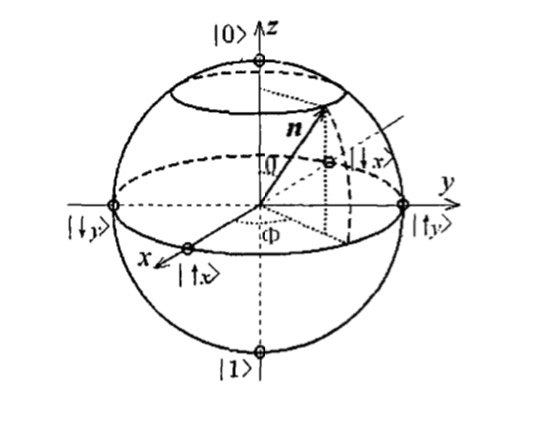
\includegraphics[width=6cm,height=5cm]{bloch.jpg}
	\caption{Blcoh vector of pure state quantum system 	}
	\end{figure}

According to Exercise 2.11, The Pauli matrix $\sigma_{X},\sigma_{Y},\sigma_{Z}$ can be written as \\
\begin{equation}
	\begin{aligned}
		\sigma_{X}=&\ket{+}\bra{+}-\ket{-}\bra{-}\\
	\sigma_{Y}=&\frac{1}{2}\left[\begin{bmatrix}1\\i\end{bmatrix}\begin{bmatrix}1 &i\end{bmatrix}
	-\begin{bmatrix}1\\-i\end{bmatrix}\begin{bmatrix}1&-i\end{bmatrix}
		\right]\\
		\sigma_{Z}=&\ket{0}\bra{0}-\ket{1}\bra{1}.\\
	\end{aligned}
\end{equation}
The eigenvectors of $\sigma_{X}$ are $\frac{1}{\sqrt{2}}(\ket{0}+\ket{1})$ and $\frac{1}{\sqrt{2}}(\ket{0}-\ket{1})$.
\\
\begin{equation}
	\begin{aligned}
		\frac{1}{\sqrt{2}}(\ket{0}+\ket{1})=&\ket{\sigma_{X}(\frac{\pi}{2},0)}\\
		=&\cos{\frac{\pi}{4}}\ket{0}+e^{i0}\sin{\frac{\pi}{4}}\ket{1}  \\
		=&\begin{bmatrix}
			\cos{\frac{\pi}{4}} \\ e^{i0}\sin{\frac{\pi}{4}}
		\end{bmatrix} \leftrightarrow \\
		n=&(\sin{\Theta}\cos{\phi},\sin{\Theta}\sin{\phi},\cos{\Theta})\\
		 =&(1,0,0)\\
		 \frac{1}{\sqrt{2}}(\ket{0}-\ket{1})=&\ket{\sigma_{X}(\frac{\pi}{2},\pi)}\\
		=&\cos{\frac{\pi}{4}}\ket{0}+e^{i\pi}\sin{\frac{\pi}{4}}\ket{1}  \\
		=&\begin{bmatrix}
			\cos{\frac{\pi}{4}} \\ e^{i\pi}\sin{\frac{\pi}{4}}
		\end{bmatrix} \leftrightarrow \\
		n=&(\sin{\Theta}\cos{\phi},\sin{\Theta}\sin{\phi},\cos{\Theta})\\
		 =&(-1,0,0)\\
	\end{aligned}
\end{equation}
The eigenvectors of $\sigma_{Y}$ are $\frac{1}{\sqrt{2}}(\ket{0}+i\ket{1})$ and $\frac{1}{\sqrt{2}}(\ket{0}-i\ket{1})$.
\\
\begin{equation}
	\begin{aligned}
		\frac{1}{\sqrt{2}}(\ket{0}+i\ket{1})=&\ket{\sigma_{Y}(\frac{\pi}{2},\frac{\pi}{2})}\\
		=&\cos{\frac{\pi}{4}}\ket{0}+e^{i\frac{\pi}{2}}\sin{\frac{\pi}{4}}\ket{1}  \\
		=&\begin{bmatrix}
			\cos{\frac{\pi}{4}} \\ e^{i\frac{\pi}{2}}\sin{\frac{\pi}{4}}
		\end{bmatrix} \leftrightarrow \\
		n=&(\sin{\Theta}\cos{\phi},\sin{\Theta}\sin{\phi},\cos{\Theta})\\
		 =&(0,1,0)\\
		 \frac{1}{\sqrt{2}}(\ket{0}-i\ket{1})=&\ket{\sigma_{Y}(\frac{\pi}{2},\frac{3\pi}{2})}\\
		=&\cos{\frac{\pi}{4}}\ket{0}+e^{i\frac{3\pi}{2}}\sin{\frac{\pi}{4}}\ket{1}  \\
		=&\begin{bmatrix}
			\cos{\frac{\pi}{4}} \\ e^{i\frac{3\pi}{2}}\sin{\frac{\pi}{4}}
		\end{bmatrix} \leftrightarrow \\
		n=&(\sin{\Theta}\cos{\phi},\sin{\Theta}\sin{\phi},\cos{\Theta})\\
		 =&(0,-1,0)\\
	\end{aligned}
\end{equation}
The eigenvectors of $\sigma_{Z}$ are $ket{0}$ and $ket{1}$.
\\
\begin{equation}
	\begin{aligned}
		\ket{0}=&\ket{\sigma_{Z}(0,\frac{\pi}{2})}\\
		=&\cos{0}\ket{0}+e^{i\frac{\pi}{2}}\sin{0}\ket{1}  \\
		=&\begin{bmatrix}
			\cos{0} \\ e^{i\frac{\pi}{2}}\sin{0}
		\end{bmatrix} \leftrightarrow \\
		n=&(\sin{\Theta}\cos{\phi},\sin{\Theta}\sin{\phi},\cos{\Theta})\\
		 =&(0,0,1)\\
		\ket{1}=&\ket{\sigma_{Z}(\pi,\frac{3\pi}{2})}\\
		=&\cos{\frac{\pi}{4}}\ket{0}+e^{i\frac{3\pi}{2}}\sin{\frac{\pi}{4}}\ket{1}  \\
		=&\begin{bmatrix}
			\cos{\frac{\pi}{2}} \\ e^{i\frac{3\pi}{2}}\sin{\frac{\pi}{2}}
		\end{bmatrix} \leftrightarrow \\
		n=&(\sin{\theta}\cos{\phi},\sin{\Theta}\sin{\phi},\cos{\Theta})\\
		 =&(0,0,-1)\\
	\end{aligned}
\end{equation}
\\
\\
\textbf{Exercise 4.2: }Let $x$ be a real number and $A$ a matrix such that $A^{2} = I$. Show that
\begin{equation}
	\begin{aligned}
		exp(iAx) = cos(x)I + isin(x)A.
	\end{aligned}
\end{equation}
Use this result to verify Equations (4.4) through (4.6).
\\
\textbf{Answer:}\\
According to Taylor series expansion formula, \\
\begin{equation}
	\begin{aligned}
		e^{x}=&1+x+\frac{x^{2}}{2!}+\frac{x^{3}}{3!}+...+\frac{x^{k}}{k!}+...;\\
		\sin{x}=&x-\frac{x^{3}}{3!}+\frac{x^{5}}{5!}-...(-1)^{k-1}\frac{x^{2k-1}}{(2k-1)!}+...;\\
		\cos{x}=&1-\frac{x^{2}}{2!}+\frac{x^{4}}{4!}-...(-1)^{k}\frac{x^{2k}}{(2k)!}+...;\\
		exp(iAx)=&I+iAx+\frac{(iAx)^{2}}{2!}+\frac{(iAx)^{3}}{3!}+...+\frac{iAx^{k}}{k!}+...;\\
				=&I+iAx-\frac{Ix^{2}}{2!}-\frac{(iA)x^{3}}{3!}+...(-1)^{(k-1)/2}\frac{iAx^{k}}{k!}+...;\\
		cos(x)I=&I-\frac{Ix^{2}}{2!}+\frac{Ix^{4}}{4!}-...(-1)^{k}\frac{Ix^{2k}}{(2k)!}+...;\\
		iAsin(x)=&iAx-\frac{iAx^{3}}{3!}+\frac{iAx^{5}}{5!}-...(-1)^{(k-1)/2}\frac{x^{2k-1}}{(2k-1)!}+...;\\
	\end{aligned}
\end{equation}
Thus we proved that $exp(iAx) = cos(x)I + iAsin(x)= cos(x)I + isin(x)A.$\\
\\
\\
\textbf{Exercise 4.3:} Show that, up to a global phase, the $\pi/8$ gate satisfies $T = R_{z}(\pi/4).$
  \\
\textbf{Answer:}\\
\begin{equation}
	\begin{aligned}
		R_{z}=&\begin{bmatrix}
			e^{-i\theta/2} & 0 \\
			0 & e^{i\theta/2} 
		\end{bmatrix} \\
		T=&e^{-i\pi/8} \begin{bmatrix}
			e^{-i\pi/8} & 0 \\
			0 & e^{i\pi/8} 
		\end{bmatrix}  \\
			R_{z}(\frac{\pi}{4})=&\begin{bmatrix}
				e^{-i \pi/8} & 0 \\
				0 & e^{i \pi/8} 
			\end{bmatrix}
	\end{aligned}
\end{equation}
Thus, up to a global phase, the  $\pi/8$ gate satisfies $T = R_{z}(\pi/4).$
 \\
\\
\textbf{Exercise 4.4: } Express the Hadamard gate $H$ as a product of $R_{x}$ and $R_{z}$ rotations and $e^{iφ} $ for some $φ$.\\
\textbf{Answer:}\\
Hardamard is rotated 90 ° around the y-axis and 180 ° around the z-axis. 
According to Trigonometric function formula, $sin(2\alpha)=2sin(\alpha)cos(\alpha)$ and $cos^{2}(\alpha)=2cos^{2}(\alpha)-1$.\\
\begin{equation}
	\begin{aligned}
		R_{x}(\theta)R_{z}(\theta)=&\begin{bmatrix}
			\cos{\theta/2}& -i\sin{\theta/2} \\  -i\sin{\theta/2} &\cos{\theta/2}
		\end{bmatrix}
		\begin{bmatrix}
			\cos{\theta/2} -i\sin{\theta/2}  & 0 \\0  i\sin{\theta/2} +\cos{\theta/2}
		\end{bmatrix}
		\\
		=&\frac{1}{2}\begin{bmatrix}
			\cos^{2}{\theta/2} -i\sin{\theta/2}\cos{\theta/2} &\cos{\theta/2} -i\sin^{2}{\theta/2}\\
			\cos{\theta/2} -i\sin^{2}{\theta/2} &\cos^{2}{\theta/2} -i\sin{\theta/2}\cos{\theta/2} \\
		\end{bmatrix}
		\\
		=&\begin{bmatrix}
			1+exp(-i\theta) &1+exp(i\theta) \\
			-1+exp(-i\theta) &1+exp(i\theta)
		\end{bmatrix} \\
		H=&\frac{X+Z}{\sqrt{2}}\\
		 =&R_{x}(\pi)R_{y}(\pi)
	\end{aligned}
\end{equation}
	\\
	\\
\textbf{Exercise 4.5: } Prove that $ (\hat{n}\cdot \vec{\sigma})^{2} = I$, and use this to verify Equation (4.8).
\\
\textbf{Answer:}\\
\begin{equation}
	\begin{aligned}
		(\hat{n}\cdot \vec{\sigma})^{2}=&\left[(n_{x},n_{y},n_{z})(\sigma_{1},\sigma_{2},\sigma_{3})\right]^{2}\\
					=&\left[n_{x}\sigma_{1}+n_{y}\sigma_{2}+n_{z}\sigma_{3}\right]^{2} \\
					=&\left(n_{x}^{2}\sigma_{1}^{2}+n_{x}n_{y}\sigma_{1}\sigma_{2}+n_{x}n_{z}\sigma_{1}\sigma_{3}
					+n_{y}^{2}\sigma_{2}^{2}+n_{y}n_{x}\sigma_{2}\sigma_{1}+n_{y}n_{z}\sigma_{2}\sigma{3} 
					\right)\\
					+&\left(n_{z}^{2}\sigma_{3}^{2}+n_{z}n_{x}\sigma_{3}\sigma_{1}+n_{z}n_{y}\sigma_{3}\sigma{2}
					\right)\\
					=&n_{x}^{2}I+in_{x}n_{y}\sigma_{3}-in_{x}n_{z}\sigma_{2}+n_{y}^{2}I-in_{y}n_{x}\sigma_{3}
					+in_{y}n_{z}\sigma_{1}+n_{z}^{2}I+in_{z}n_{x}\sigma_{2}-in_{z}n_{y}\sigma_{1}\\
					=&I(n_{x}^{2}+n_{y}^{2}+n_{z}^{2})=I\\
				R_{\hat{n}}(\theta)\equiv &exp(-i\theta\hat{n}\cdot\sigma/2) \\
				=&cos(\frac{\theta}{2})I-isin(\frac{\theta}{2})\theta\hat{n}\cdot\sigma\\
				=&cos(\frac{\theta}{2})I-isin(\frac{\theta}{2})(n_{x}X+n_{y}Y+n_{z}Z) \\
	\end{aligned}
\end{equation}
\\
\\
\textbf{Exercise 4.6: (Bloch sphere interpretation of rotations) } One reason why the $R_{\hat{n}}(\theta)$ operators are 
referred to as rotation operators is the following fact, which you are to prove. Suppose a single qubit 
has a state represented by the Bloch vector $\vec{\lambda}$. Then the effect of the rotation  $R_{\hat{n}}(\theta)$  on the state is 
to rotate it by an angle $\theta$ about the $\hat{n} $ axis of the Bloch sphere. This fact explains the rather mysterious 
looking factor of two in the definition of the rotation matrices.
\\
\textbf{Answer:}\\
\\
\\
\textbf{Exercise 4.7: } Show that $XYX = −Y$ and use this to prove that $XR_{y}(\theta)X = R_{y}(−\theta)$.
\\
	\textbf{Answer:}\\
	\begin{equation}
		\begin{aligned}
			XYX=&\begin{bmatrix}
				0 & 1 \\ 1 &0
			\end{bmatrix}
			\begin{bmatrix}
				 0 &-i \\ i & 0
			\end{bmatrix}
			\begin{bmatrix}
				0 & 1 \\ 1 & 0	
			\end{bmatrix} \\
			=&\begin{bmatrix}
				 i & 0	\\ 0 & -i 
			\end{bmatrix}
			\begin{bmatrix}
				0 & 1 \\ 1 & 0	
			\end{bmatrix} \\
			=&\begin{bmatrix}
				0 &i \\ -i & 0
			\end{bmatrix} =-Y \\
			XR_{y}(\theta)X=&\begin{bmatrix}
				0 & 1 \\ 1 &0
			\end{bmatrix}
			\begin{bmatrix}
			cos(\frac{\theta}{2}) &-sin(\frac{\theta}{2})	 \\ sin(\frac{\theta}{2})    &cos(\frac{\theta}{2})
			\end{bmatrix}
			\begin{bmatrix}
				0 & 1 \\ 1 &0
			\end{bmatrix}
			=&\begin{bmatrix}
				sin(\frac{\theta}{2})	&cos(\frac{\theta}{2}) \\ cos(\frac{\theta}{2}) &-sin(\frac{\theta}{2})	
			\end{bmatrix}
			\begin{bmatrix}
				0 & 1 \\ 1 &0
			\end{bmatrix}\\
			=& \begin{bmatrix}
				cos(\frac{\theta}{2}) &sin(\frac{\theta}{2})	\\	-sin(\frac{\theta}{2})	&cos(\frac{\theta}{2})
			\end{bmatrix}
			\\
			R_{y}(-\theta)=&e^{i\theta Y/2} \\ 
			=&cos(\theta/2)I+isin(\theta/2)Y  \\
			=&\begin{bmatrix}
				cos(\theta/2) &0\\0 &cos(\theta/2)
			\end{bmatrix}+
			\begin{bmatrix}
			0 & sin(\theta/2)\\ -sin(\theta/2) &0 
			\end{bmatrix} \\
			=&\begin{bmatrix}
				cos(\frac{\theta}{2}) &sin(\frac{\theta}{2})	\\	-sin(\frac{\theta}{2})	&cos(\frac{\theta}{2})
			\end{bmatrix}
		\end{aligned}
	\end{equation}
	Thus, we proved that $XR_{y}(\theta)X = R_{y}(−\theta)$.
	\\
\\
\textbf{Exercise 4.8: } An arbitrary single qubit unitary operator can be written in the form \\
\begin{equation}
	\begin{aligned}
		U = exp(i\alpha)R_{\hat{n}} (\theta)
	\end{aligned}
\end{equation}
for some real numbers $\alpha$ and $\theta$, and a real three-dimensional unit vector $\hat{n}$.
\begin{enumerate}[1.]
	\item Prove this fact.
	\item Find values for $\alpha$ , $\theta$, and $\hat{n}$ giving the Hadamard gate $H$.
	\item Find values for $\alpha$ , $\theta$, and $\hat{n}$ giving the phase gate 
	\begin{equation}
		\begin{aligned}
			S=\begin{bmatrix}
				1 & 0 \\ 0 & i
			\end{bmatrix}
		\end{aligned}
	\end{equation}
\end{enumerate}
\textbf{Answer:}\\
\begin{enumerate}[1.]
	\item \begin{equation}
		\begin{aligned}
			exp(i\alpha)R_{\hat{n}} (\theta)=&exp(i\alpha)exp(-i\theta\hat{n}\cdot\sigma/2) \\
											=&(cos(\alpha)+isin(\alpha))(cos(\frac{\theta}{2})I-isin(\frac{\theta}{2})(n_{x}X+n_{y}Y+n_{z}Z)) \\
		\end{aligned}
	\end{equation}
	\item $ U=exp(i\alpha)R_{\hat{n}}(\theta)=\begin{bmatrix}
		U_{11} & U_{12} \\  U_{21} & U_{22}
	\end{bmatrix}$, among then,
	\\
	\begin{equation}
		\begin{aligned}
			U_{11}=&\left(cos \alpha cos(\frac{\theta}{2})+n_{z}sin\alpha sin(\frac{\theta}{2})\right)
			+i\left(sin \alpha cos(\frac{\theta}{2})-n_{z}cos\alpha sin(\frac{\theta}{2}) \right) \\
			U_{12}=&\left(n_{x}sin \alpha sin(\frac{\theta}{2})-n_{y}cos\alpha sin(\frac{\theta}{2})\right)\\
			-i\left(n_{x}cos \alpha sin(\frac{\theta}{2})+n_{y}sin\alpha sin(\frac{\theta}{2}) \right)\\
            U_{21}=&\left( n_{x}sin \alpha sin(\frac{\theta}{2})+n_{y}cos\alpha sin(\frac{\theta}{2})\right)
            -i\left(n_{x}cos \alpha sin(\frac{\theta}{2})-n_{y}sin\alpha sin(\frac{\theta}{2}) \right) \\
            U_{22}=&\left( cos \alpha cos(\frac{\theta}{2})-n_{z}sin\alpha sin(\frac{\theta}{2})\right)
            +i\left(sin \alpha cos(\frac{\theta}{2})+n_{z}cos\alpha sin(\frac{\theta}{2}) \right) \\
			H=&\frac{1}{\sqrt{2}}\begin{bmatrix}
                1 &0\\ 0 & -1
            \end{bmatrix}
			\\
			U_{11}=&\frac{1}{\sqrt{2}}, U_{12}=0\\
			U_{21}=&0, U_{22}=-\frac{1}{\sqrt{2}}\\
		\end{aligned}
	\end{equation}
	The solution is $\alpha=\frac{\pi}{2}, \theta=\pi, \hat{n}=\frac{1}{\sqrt{2}}(1,0,1)$, then \\
		$H=exp(\frac{i\pi}{2})R_{\hat{n}}(\pi)$, for $\hat{n}=\frac{1}{\sqrt{2}}(1,0,1)$. 
	\\
	\item $	S=\begin{bmatrix}1 & 0 \\ 0 & i \end{bmatrix} $, then \\
	 $U_{11}=\frac{1}{\sqrt{2}}, U_{12}=0$\\
	$ U_{21}=0, U_{22}=-\frac{i}{\sqrt{2}}$.\\
	The solution is $ \alpha=\frac{\pi}{4}, \theta=\pi, \hat{n}=\frac{1}{\sqrt{2}}(0,0,1)$, then \\
	$S =exp(\frac{i\pi}{4})R_{\hat{n}}(\pi)$, for $\hat{n}=\frac{1}{\sqrt{2}}(0,0,1)$.
\end{enumerate}
\textbf{Exercise 4.9: } Explain why any single qubit unitary operator may be written in the form (4.12).
\\
\textbf{Answer:}\\
\\
\\
\textbf{Exercise 4.10: ($X-Y$ decomposition of rotations) }   Give a decomposition analogous to Theorem 4.1 
but using $R_{x}$ instead of $R_{z}$.
 \\
\textbf{Answer:}	 \\
\begin{equation}
	\begin{aligned}
		U=&\begin{bmatrix}
			exp(i(\alpha-\frac{\beta}{2}-\frac{\delta}{2}))cos(\frac{\gamma}{2}) &
		-exp(i(\alpha-\frac{\beta}{2}+\frac{\delta}{2}))sin(\frac{\gamma}{2}) \\
		exp(i(\alpha+\frac{\beta}{2}-\frac{\delta}{2}))sin(\frac{\gamma}{2}) &
		exp(i(\alpha+\frac{\beta}{2}+\frac{\delta}{2}))cos(\frac{\gamma}{2})
	\end{bmatrix}
	\\
	=&exp(i\alpha)\begin{bmatrix}
		cos(\frac{\beta}{2})-isin(\frac{\beta}{2}) & 0\\
		0 & cos(\frac{\beta}{2})+isin(\frac{\beta}{2})
	\end{bmatrix}
	\begin{bmatrix}
		cos(\frac{\gamma}{2}) & sin(\frac{\gamma}{2}) \\
		sin(\frac{\gamma}{2}) &cos(\frac{\gamma}{2})
	\end{bmatrix}
	\begin{bmatrix}
		cos(\frac{\delta}{2})-isin(\frac{\delta}{2}) & 0\\
		0 & cos(\frac{\delta}{2})+isin(\frac{\delta}{2})
	\end{bmatrix}
	\\
	\end{aligned}
\end{equation}

\end{quote}
\end{document}